	\chapter{Ο πηρύνας της Μηχανής}
	
	Ένα framework το οποίο επεκτείνεται και διακλαδώνεται σε πολλές υπο-βιβλιοθήκες, στηρίζεται στη θεμελιώση ενός framework core, του πηρύνα της βιβλιοθήκη. Το \gls{API} του πηρύνα πρέπει να είναι εύκολο στην κατανόηση, να αποτελείται από αυτοεπεξηγούμενες αφαιρέσεις, οι οποίες εκθέτουν μόνο τα απολύτος απαραίτητα, ώστε οι υποβιβλιοθήκες που χρησιμοποιούν τον πηρύνα να μην δεσμεύονται σε υλοποιήσεις, να περιορίζει σε συγκεκριμένο pipeline χρήσης για αποφυγή απρόβλεπτων συμπεριφορών και να προσφέρει δυνατότητες επεκτασιμότητας.  \cite{jaroslav08}
		
	\begin{theorem}[First test theorem]
		This is a test theorem.
	\end{theorem}

	\section{Κύκλος ζωής πηρύνα}	
	Κάθε οντότητα από τη στιγμή της δημιουργίας της στο περιβάλλον της μηχανής μέχρι την καταστροφής της και διαγραφή της από την μνήμη, περνά από κάποια προκαθορισμένα στάδια τα οποία εκτελούνται ανάλογα με την κατάσταση του υλικού και του λογισμικού.
	
	\begin{itemize}
		\item Initialization εκτελείται μόνο κατά τη δημιουργία
		\item Game loop εκτελείται συνέχεια σε βρόγχο
		\item Disposing εκτελείται κατά την καταστροφή
	\end{itemize}
	
	\begin{figure}[h!]
		\centering
		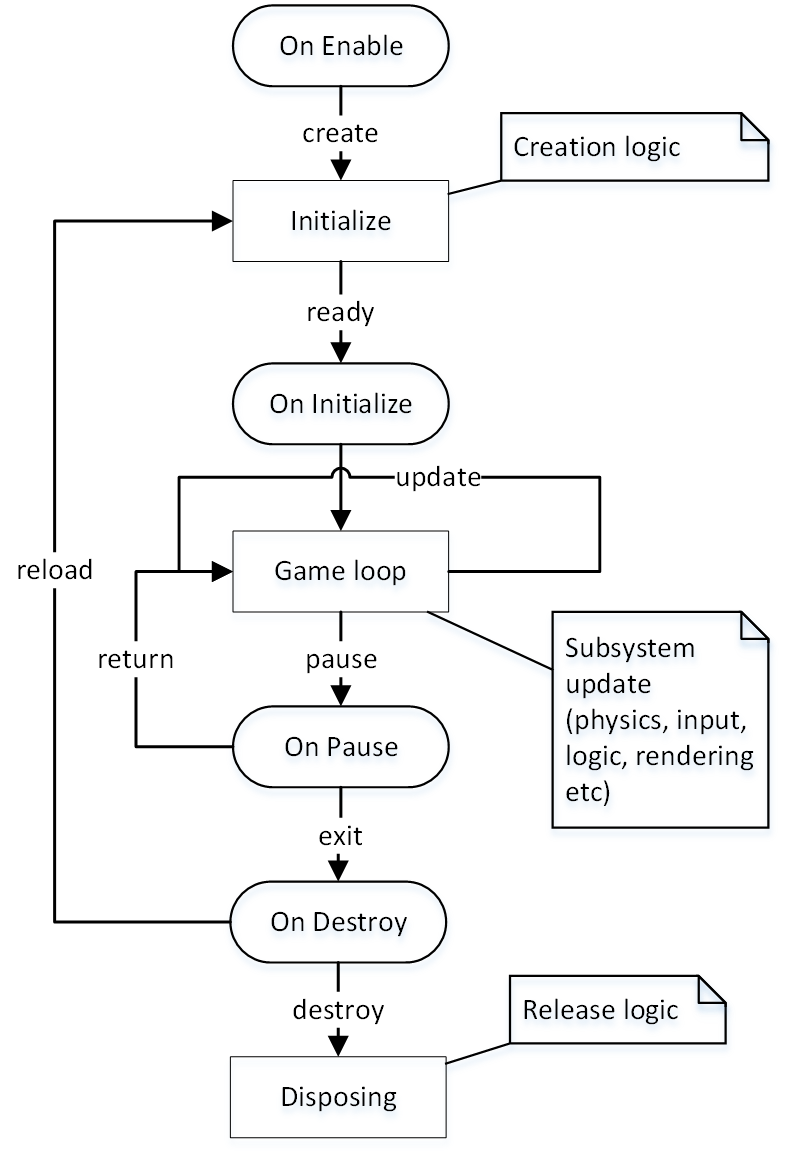
\includegraphics[width=80mm]{Images/core_lifecycle}
		\caption{Core Lifecycle}
		\label{fig:corelifecycle}
	\end{figure}
		
	\subsection{Game Loop}
	To game loop εγκυάται τη συνεπής ενημέρωση των υποσυστημάτων ανάλογα με το προκαθορισμένο χρονικό βήμα. Χωρίς το ανεξάρτητο σύστημα ενημέρωσης υποσυστημάτων, η ενημέρωση θα γινόταν στον κύκλο εκτέλεσης του επεξεργαστή με αποτέλεσμα την διαφορετική εμπειρία ανά επεξεργαστή και μηχάνημα.
	
	Το κάθε υποσύστημα έχει διαφορετικές απαιτήσεις για τη βέλτιστη λειτουργία. Το collision detection system μπορεί να χρειάζεται να ενημερώνεται εκατό φορές το δευτερόλεπτο, ενώ το σύστημα τεχνητής νοημοσύνης δύο φορές το δευτερόλεπτο. Η πιο συνηθισμένη τεχνική είναι να υπάρχουν δύο κύρια update loops
	\begin{itemize}
	\item το game loop στο οποίο ενημερώνονται όλα τα υποσυστήματα, physics, logic, dynamics κλπ
	\item rendering loop στο οποίο γίνονται οι κλήσεις στην κάρτα γραφικών και τρέχει στα 50-60 \gls{FPS}
	\end{itemize}
	
	Η διαφορά του χρόνου μεταξύ των ενημερώσεων πρέπει να είναι εγγυημένη για παράδειγμα σε μια μηχανή στην οποία το rendering loop τρέχει στα 60 \gls{FPS} υπάρχει η συχνότητα ενημέρωσης
	\begin{equation}
	 F = 1/T =>  F = 1000ms/60 => F = 16ms. 
	\end{equation}Για να μπορεί να εγγυάται το σύστημα αυτή την αναλογία, πρέπει να μετράει τη διαφορά χρόνου μεταξύ κάθε κλήσης, να εκτελεί τον κώδικα στο συγκεκριμένο loop και για τον υπόλοιπο χρόνο το thread να κοιμάται.
	
	Στα συστήματα πραγματικού χρόνου, η έννοια της διάρκειας και του χρόνου πρέπει να χειρίζεται ως μια ξεχωριστή οντότητα. Ο χρόνος πρέπει να είναι ανεξάρτητος από τον πραγματικό χρόνο. Ένα animation το οποίο γίνεται render σε πραγματικό χρόνο, μπορεί να παίξει αντίστροφα ή με διπλάσια ταχύτητα, αν το χρονοδιάγραμμα στο οποίο ανταποκρίνεται, χειρίζεται τον χρόνο διαφορετικά.
	Όλα τα συστήματα ενημερώνονται γραμμικά συναρτήσει του χρόνου του οποίο παρέχεται ως είσοδος.
	
	\subsection{Υποσυστήματα}
	Το κάθε υποσύστημα δημιουργείται ενημερώνεται και καταστρέφεται μέσα στο γενικό κύκλο ζωής του πηρύνα. Το κάθε υποσύστημα έχει εσωτερικά το δικό του κύκλο ζωής και κύκλο ενημέρωσης ο οποίος λειτουργεί μέσα στην έκταση του εξωτερικού κύκλου ζωής.
	
	\subsection{Τεχνικές Ενημέρωσης Υποσυστημάτων}
	Τα υποσυστήματα με κάποιο τρόπο πρέπει να ενημερώνονται και να επικοινωνούν μεταξύ τους ή να στέλνουν μηνύματα όταν συμβεί κάποιο γεγονός. Υπάρχουν διάφορές τεχνικές ενημέρωσης υποσυστημάτων.
	\begin{itemize}
	\item Message Pumps: τα υποσυστήματα στέλνουν μηνύματα σε ένα message bus και τα συστήματα ενημερώνονται όταν εξυπηρετείται το μήνυμα. Παραμένουν άεργα εφόσον δεν υπάρχει μήνυμα προς εξυπηρέτηση.
	\item Call-back driven: τα υποσυστήματα παρέχουν call-back λειτουργικότητα. Δηλαδή τη δυνατότητα να θέσεις τι κώδικας θα εκτελεστεί κατά κάποιο συμβάν. Ένα συμβάν μπορεί να είναι η σύγκρουση μεταξύ δύο αντικειμένων. Ο χρήστης μπορεί να πει ότι όταν συμβεί σύγκρουση μεταξύ του παίχτη και του εχθρού, ο παίχτης θα χάσει ζωή.
	\end{itemize}
	
	\begin{figure}[h!]
		\centering
		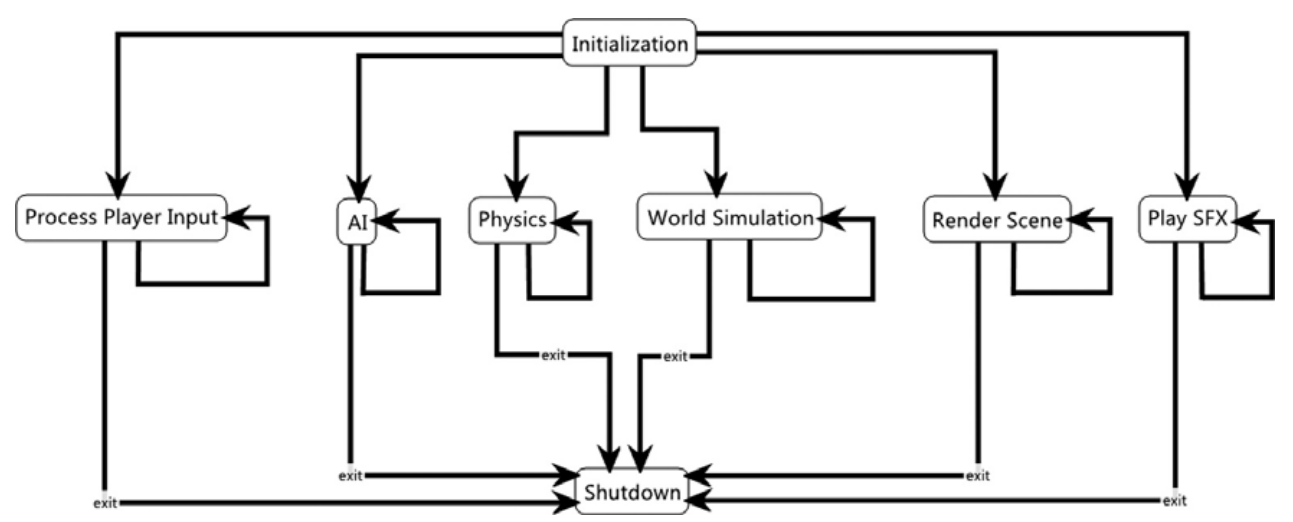
\includegraphics[width=160mm]{Images/game_coding_complete_chapter7_gameloops}
		\caption{game loops}
		\label{fig:gameloops}
	\end{figure}
		
	\section{ScreenSystem}
	Σε ένα τυπικό χρόνο εκτέλεσης ενός παιχνιδιού, το παιχνίδι περνά από διάφορες καταστάσεις. Οι καταστάσεις αυτές μπορεί να είναι η προσωρινή παύση, ένα μενού ρυθμίσεων ένα \gls{GUI} επιλογών το οποίο επικαλύπτει το τρέχον παιχνίδι ή απoδίδεται στον ίδιο render buffer. Το παιχνίδι χωρίζεται σε σκηνές, σε επίπεδα και σε χάρτες οι οποίες έχουν ξεχωριστό τρόπο απόδοσης στην οθόνη. Μία σκηνή μπορεί να αποδίδεται από διάφορες υποσκηνές οι οποίες δίνουν την ψευδαίσθηση του βάθους στο φόντο. Η σειρά απόδοσης των σκηνών πρέπει να είναι ρυθμιζόμενη και ελεγχόμενη. Η κάθε σκηνή μπορεί να παρομοιαστεί ως μια οθόνη.

	\subsection{Απαιτήσεις}
	Ο χρήστης του συστήματος έχει πλήρη έλεγχο της κάθε οθόνης-σκηνής και προσαρμόζει τη λογική και την απόδοση ανάλογα. Το κεντρικό σύστημα διαχείρισης προσφέρει τη δυνατότητα προετοιμασίας οθονών, αναζήτησης μέσω κλειδιών, αυτόματη διαχείριση και εναλλαγή και εξατομίκευση τους. Για τη διατήρηση της συνοχή κατά την εναλλαγή οθόνων, προσφέρεται η δυνατότητα εξατομίκευσης της απόδοσης κατά τις μεταβάσεις.

	\begin{figure}[h!]
		\centering
		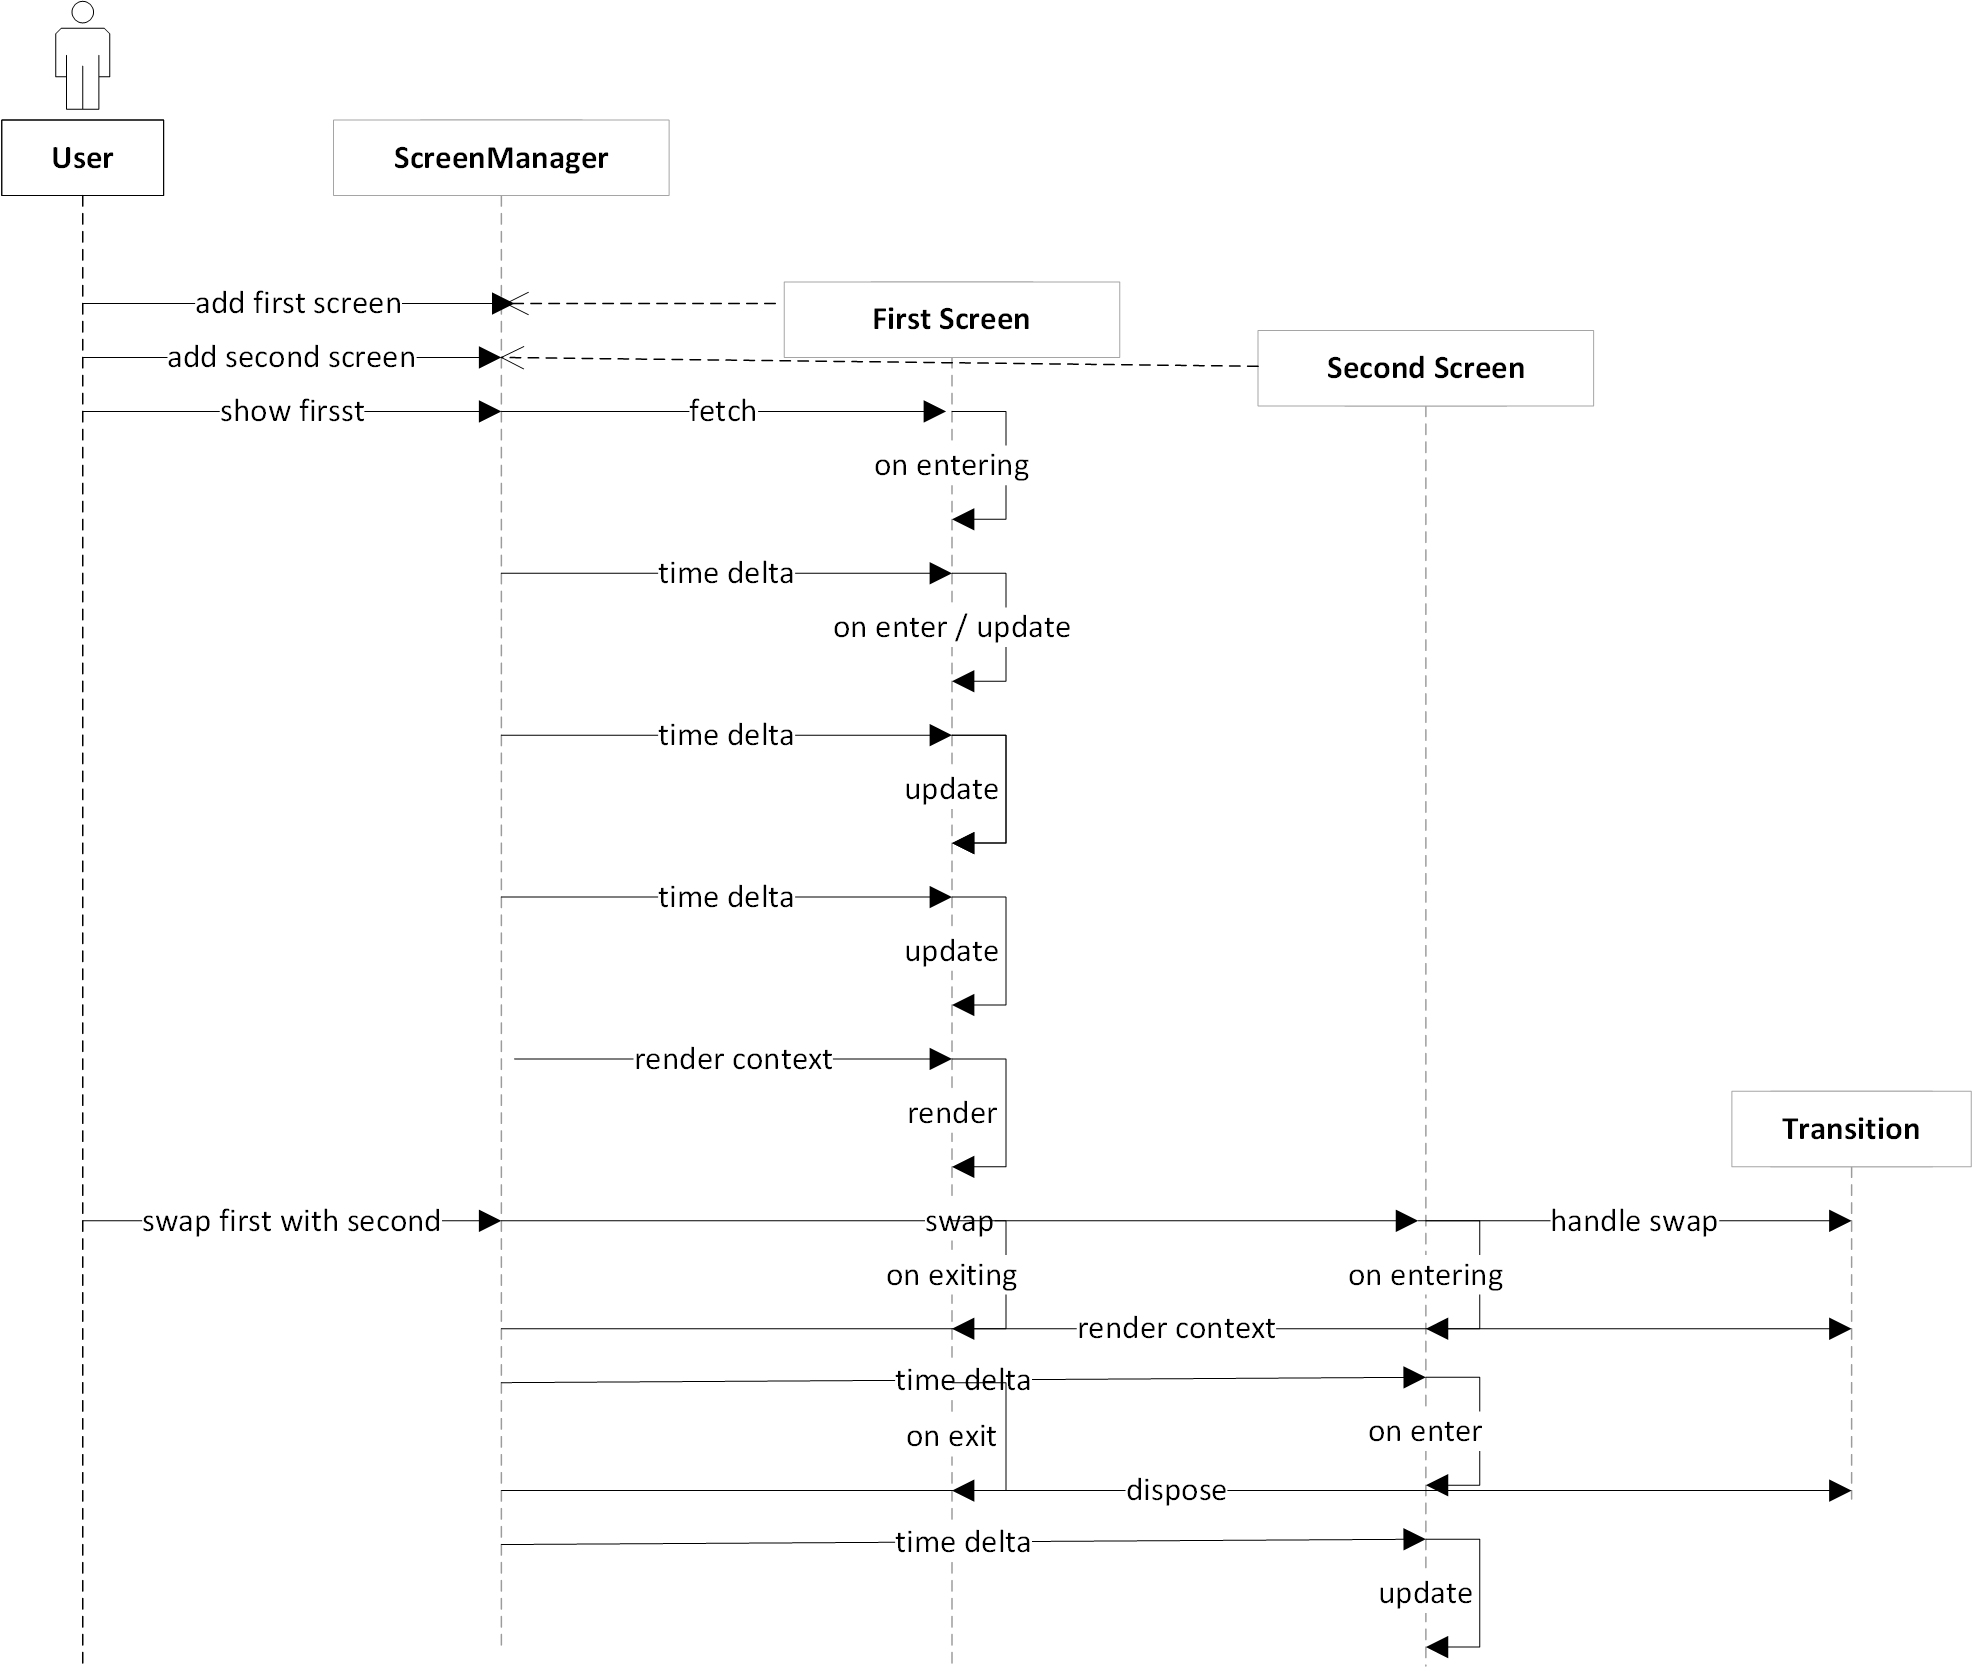
\includegraphics[width=165mm]{Images/screensystem_sequence}
		\caption{screensystem sequence}
		\label{fig:screensystem_sequence}
	\end{figure}	
	
	\subsection{Συστατικά του συστήματος}		
	\paragraph{Κεντρικό σύστημα διαχείρισης}
	Οι λειτουργίες του συστήματος.
	\begin{itemize}
	\item Απόδοση και ενημέρωσης 1-N σκηνών με δυναμικά εναλλασσόμενη σειρά στο πλαίσιο του κύκλου ζωής του πηρύνα.
	\item Προετοιμασία των οθονών και δυνατότητα εύρεσης χρησιμοποιώντας κλειδιά.
	\item Εύκολη προβολή, απόκριψη, εναλλαγή οθονών χρησιμοποιώντας κλειδιά.
	\item Δυνατότητα εξατομίκευσης της απόδοσης κατά τις διάφορες μεταβάσεις των σκηνών.
	\end{itemize}

	\paragraph{Screen host}
	\begin{itemize}
		\item Παραμετροποίηση συμβάντων κατά τις αλλαγές κατάστασης
		\item Προσαρμοσμένη λογική και απόδοση 
		\item Εντολές αλλαγής κατάστασης
		\item Εξατομίκευση απόδοσης κατά την εναλλαγή κατάστασης
	\end{itemize}
	
	\paragraph{Εναλλαγή οθονών}
	Η εξατομίκευση και παραμετροποίηση της εναλλαγής οθονών λαμβάνει μέρος μέσα στο γενικό πλαίσιο απόδοσης οθονών. Ο εξατομικευτής αναλαμβανει την απόδοση του screen buffer στον οποίο αποδόθηκε η οθόνη, την κατάσταση στην οποία βρίσκεται η οθόνη, την κατεύθυνση και το ποσοστό εξέλιξης της εναλλαγής. 
			
	\lstset
	{
		style=sharpc, 
		caption={Transition Delegate}
	}
	\begin{lstlisting}	
delegate void TransitionRenderAction(ScreenState state, float progress, RenderTarget2D renderTarget, SpriteBatch batch);
	\end{lstlisting}
	
	
	\subsection{Αρχιτεκτονική}
	\begin{figure}[h!]	
		\centering
		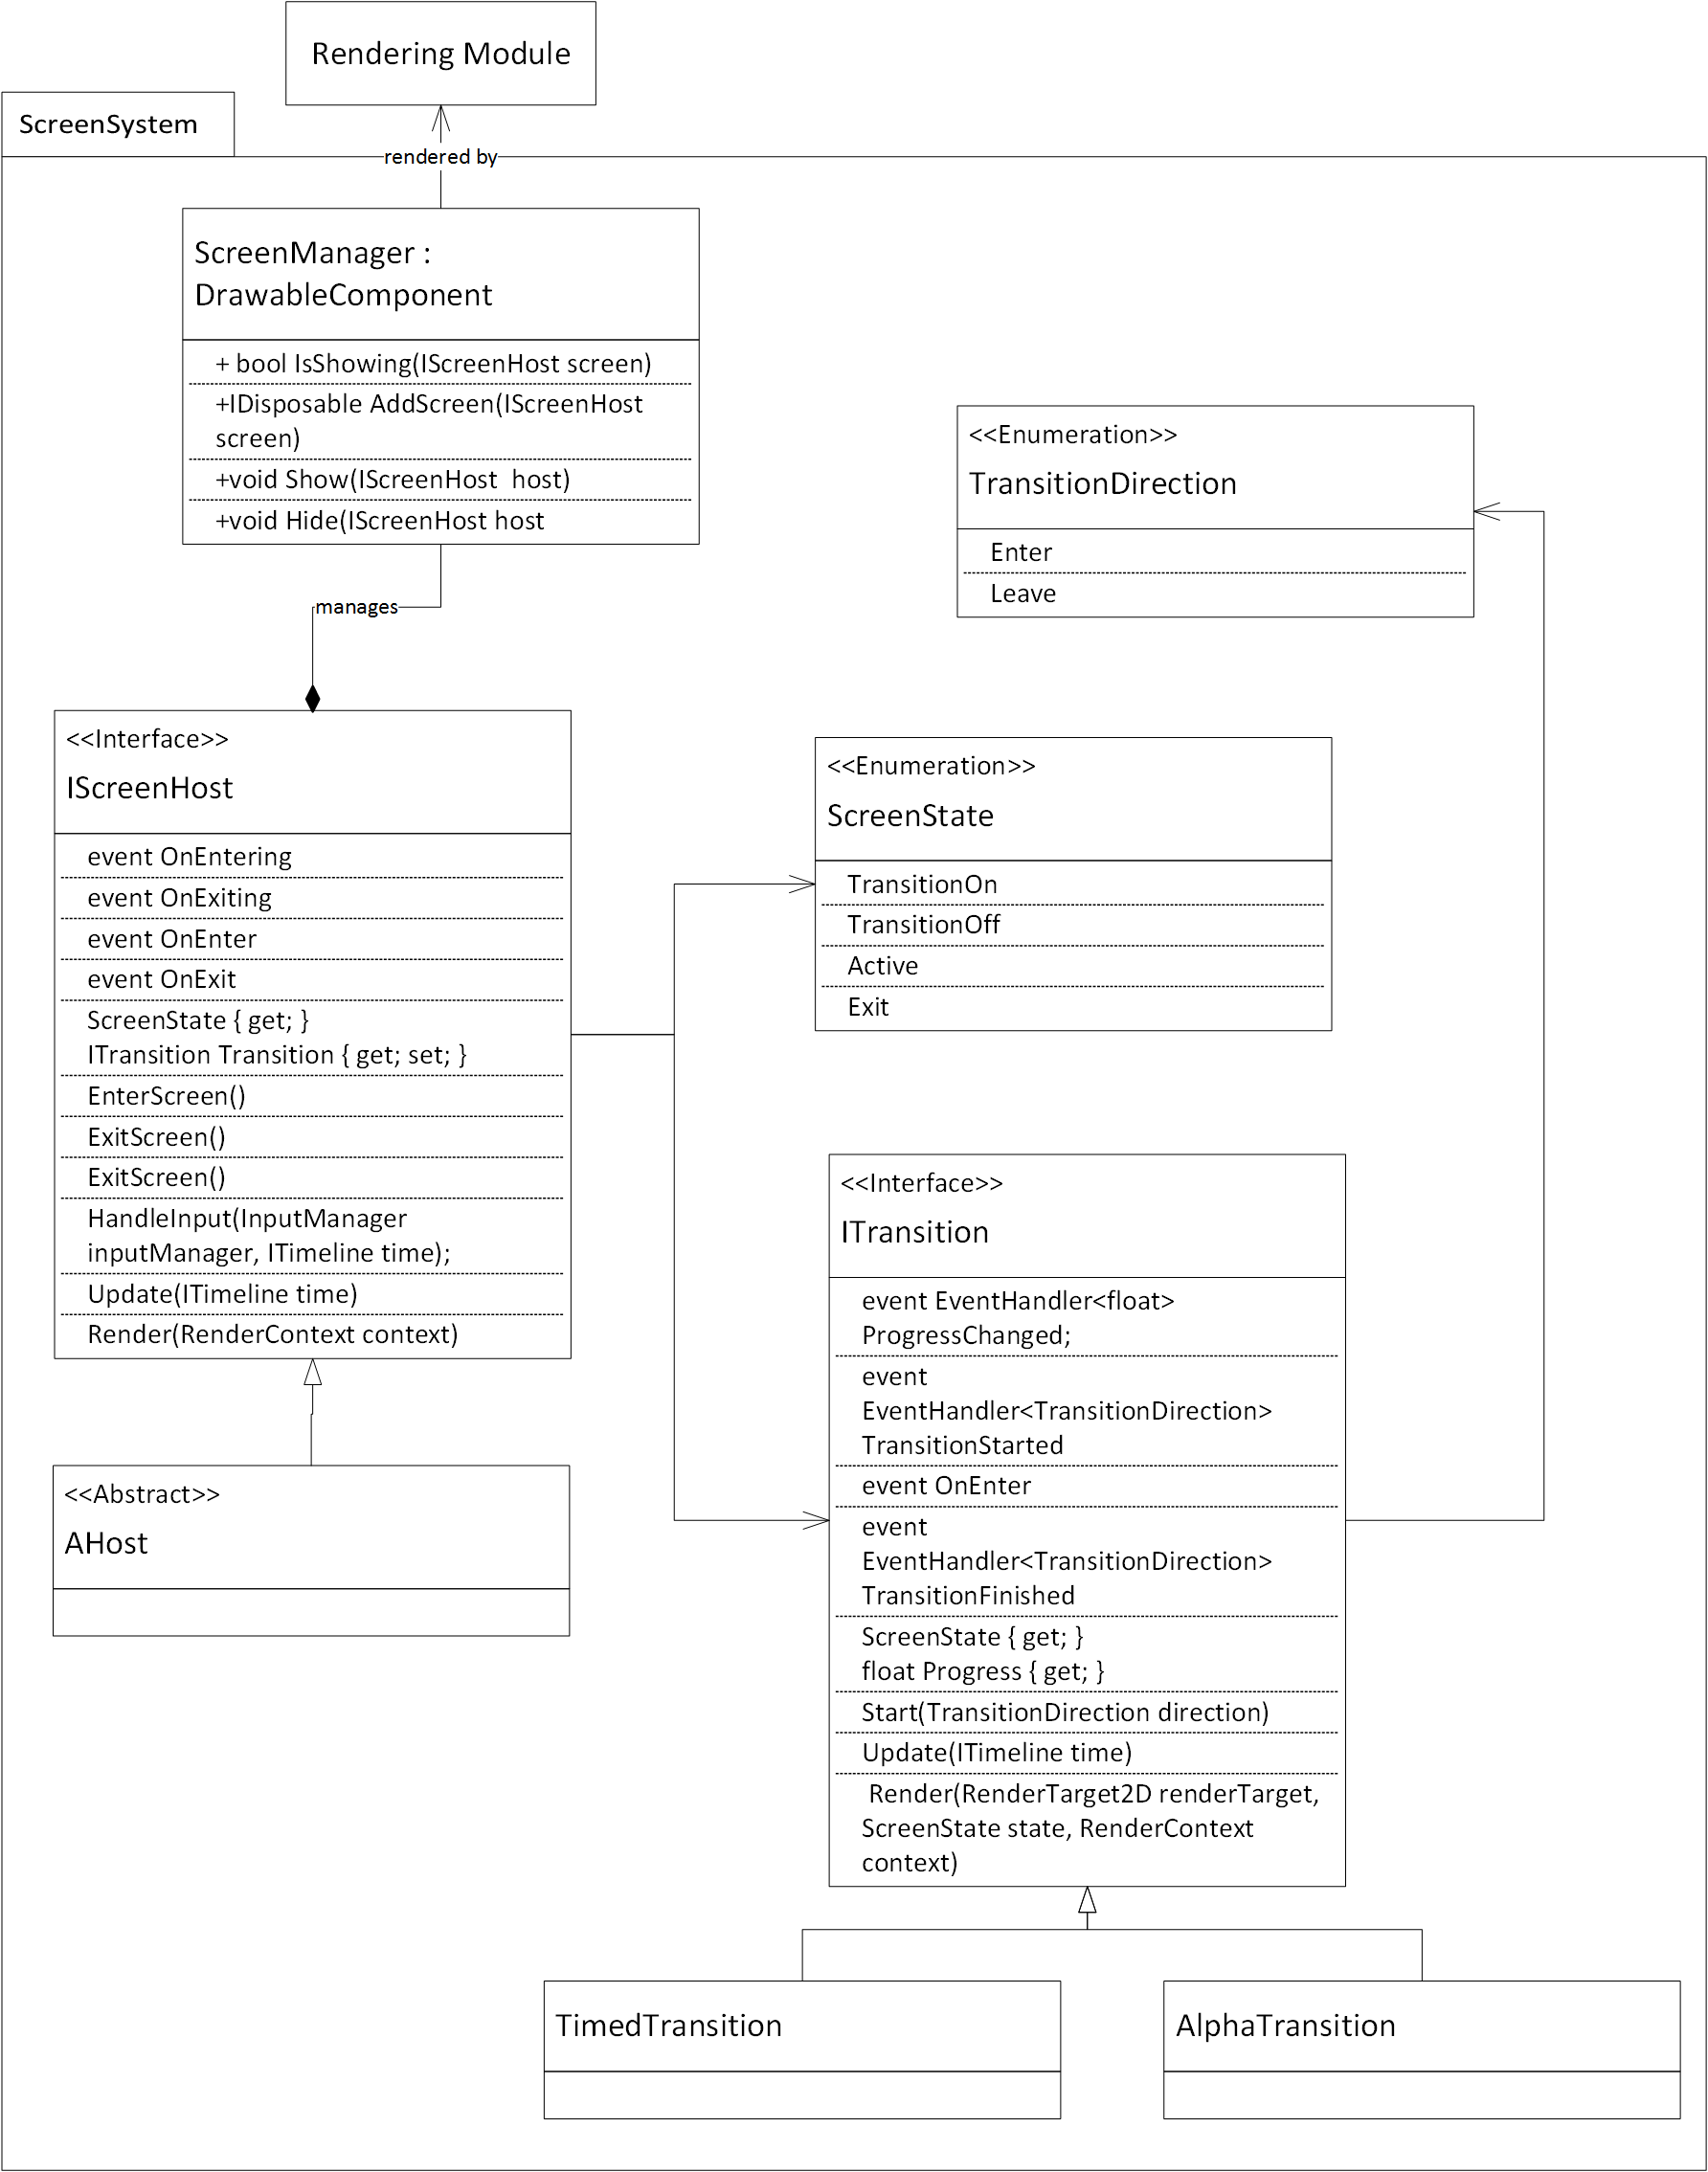
\includegraphics[width=160mm]{Images/core_screensystem}
		\caption{core screensystem}
		\label{fig:core_screensystem}
	\end{figure}		
	
	\subsection{Παράδειγματα χρήσης API}

	\lstset
	{
		style=sharpc, 
		caption={Transition Delegate}
	}
	\begin{lstlisting}
screenHost
.AddScreen(
	"FirstScreen",
	() => new MyFirstScreen());
		
screenHost["FirstScreen"]
.Show()
.Transition(
	Transition.WithTime(
         TimeSpan.FromSeconds(0.5),
         (state, progress, target, context) =>
         context.Batch.Draw(target, 
         (float)Math.Pow(progress - 1.0f, 2) * context.ScreenWidth, 
         Color.White * progress
    )
);
     
screenHost["FirstScreen"]
.Hide();   
	\end{lstlisting}
	\section{Input System}
	\subsection{Human Interface devices}
	Η μηχανή πρέπει να είναι σε θέση να διαβάζει, να επεξεργάζεται και να χρησιμοποιεί συσκευές ανθρώπινης διεπαφής. Η διαδικασία ανάγνωσης χωρίζεται στις παρακάτω κατηγορίες:
	\begin{itemize}
	\item Polling: η κατάσταση κάποιον συσκευών (κυρίως της παλιάς σχολής) διαβάζεται ρωτώντας τη συσκευή για την κατάστασή της περιοδικά. Αυτό καταλήγει σε πλεονασμό γιατί ρωτάει πολλές φορές χωρίς να παίρνει απάντηση και με μικρή καθυστέρηση γιατί η αλλαγή κατάστασης μπορεί να γίνει μεταξύ ερωτήσεων.
	\item Interrupts (διακοπές): Οι συσκευές στέλνουν δεδομένα μόνο όταν αλλάξει η κατάσταση με κάποιο τρόπο. Ο χρήστης μπορεί γράψει κώδικα και να τον εγγράψει με τρόπο ώστε να εκτελείται μόνο όταν συμβεί κάποια αλλαγή κατάστασης.
	\end{itemize}
	
	\subsection{Τύποι Input}
	
	\begin{itemize}	
	\item Digital Buttons: τα ψηφιακά κουμπιά έχουν δύο καταστάσεις: pressed / not pressed
	\item Analog axes and buttons: τα αναλογικά επιστρέφουν εύρος τιμών: το βαθμό της πίεσης της σκανδάλης ή τη θέση του μοχλού στο δισδιάστατο άξονα. 
	\item Relative Axes: οι αναφορικοί άξονες επιστρέφουν τιμές σε σχέση με το τελευταίο σημείο στο οποίο έγινε κάποια αλλαγή πχ το ποντίκι επιστρέφει τη διαφορά θέσης σε σχέση με το τελευταίο σημείο στο οποίο μετακινήθηκε.
	\item Accelerators: Ανιχνεύουν τρισδιάστατες επιταχύνσεις.
	\item Sensor bars: Αισθητήρες όπως οι κάμερες.
	\end{itemize}
	
	\subsection{Απαιτήσεις υποσυστήματος}
	Η οντότητα θέλει να εκτελέσει κώδικα προσανατολισμένο κατά συμβάν εισόδου από συσκευή ανθρώπινης διεπαφής. Ο κώδικας αυτός εκτελείται αντίστοιχα για keyboard-mouse και για gamepad. O χρήστης μπορεί να αλλάξει συσκευή διεπαφής ενώ βρίσκεται σε τρέχον παιχνίδι. Η βιβλιοθήκη δεν πρέπει να στηρίζεται σε κανένα υλικό ή συσκευή. 
	
	\subsection{Observers-listeners}
	Το κάθε υποσύστημα διαχείρισης συσκευών ανθρώπινων διεπαφών αποτελείται από τον διαχειριστή για παράδειγμα τον MouseListener ή Keyboard listener, το οποίο χρησιμοποιεί τις βιβλιοθήκες του τρέχον λειτουργικού για την επιστολή συμβάντων των διεπαφών. Ανάλογα με την πλατφόρμα στην οποία έγινε compile δημιουργούνται οι αντίστοιχοι listeners μέσω του abstract factory.
	Ο χρήστης μπορεί να προσκολήσει κώδικα ο οποίος να εκτελείται ανά συμβαν π.χ. στη μετακίνηση του ποντικιού. Οι listeners ανάλογα με τις συνθήκες επιστολής, όπως το δέλτα του χρόνου επιστολής συμβάντος διπλού click ειναι 200ms, αποστέλλουν τα συμβάντα στoυς καταχωρημένους εκτελεστές. Το κεντρικό σύστημα διαχείρισης εισόδου ενημερώνει όλες τις συνδεδεμένες συσκευές εισόδου. 
	Ο εκτελέσιμος κώδικας μπορεί να γραφτεί μια φορά, ανεξαρτήτως συμβάντος, και να προσκοληθεί στο initialization του lifecycle σε υποσυστήματα διεπαφών.
	
	\begin{figure}[h!]
		\centering
		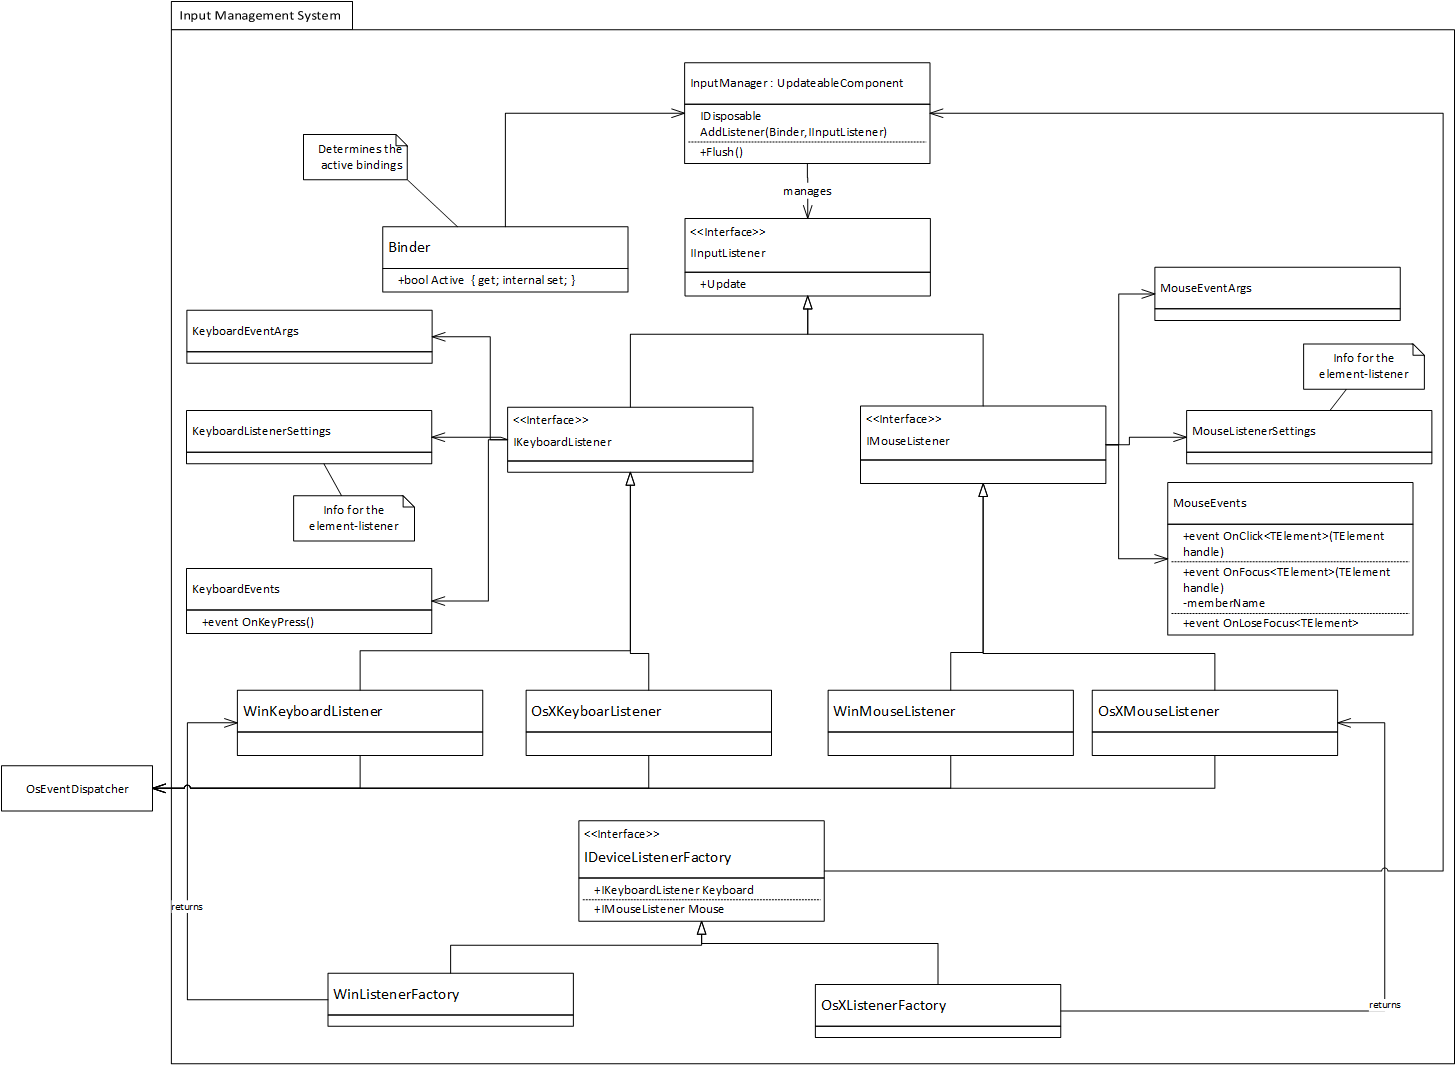
\includegraphics[width=165mm]{Images/core_input}
		\caption{core input architecture}
		\label{fig:core_input}
	\end{figure}
		
	\lstset
	{
		style=sharpc, 
		caption={Παράδειγμα listener στο initialization}
	}
	\begin{lstlisting}
inputManager.AddListener(factory => factory.GamepadListener
{
	Settings = MouseSettings
		    .DoubleClickDelta(Timespan.FromSeconds(0.2))
			.DragDelta(Timespan.FromSeconds(0.2)),
	Events   = MouseEvents
	        .OnLeftClick(sender,args) => this.Shoot())
	        .OnLeftDoubleClick(sender,args) => this.Roll())      	
});

inputManager.AddListener(factory => factory.GamepadListener
{
	Settings = GamepadSettings.Default,
	Events   = GamepadEvents
			.OnXButtonPress(sender,args) => this.Shoot())
			.OnYButtonPress(sender,args) => this.Roll())      	
});
\end{lstlisting}

\section{Physics}
Η φυσική στα παιχνίδια έχουν ως βάση τα μαθηματικά. Η ανάλυση του συστήματος της φυσικής επικεντρώνεται σε μοντελοποίηση υψηλού επιπέδου. Η υλοποίησή τους βασίζεται υλοποίηση μαθηματικών λειτουργιών γεωμετρίας, γραμμικής άλγεβρας και κινηματικής.

\subsection{Τα παιχνίδια ως soft real-time simulations}
Οι επιστήμονες αποκαλούν τα παιχνίδια soft real-time interative agent-based computer simulations.
Στα περισσότερα παιχνίδια ένα υποσύστημα του πραγματικού κόσμου μοντελοποιείται μαθηματικά, ώστε να μπορεί να αναπαραχθεί και να χειριστεί από τον υπολογιστή. 
Ενα agent-based simulation είναι μια προσομοίωση η οποία περιγράφει πως αλληλεπιδρούν τα διάφορα αντικείμενα και χαρακτήρες μέσα στον κόσμο.
Όλα τα αλληλεπιδραστηκά παιχνίδια είναι temporal simulations δηλαδή ο το μοντέλο του εικονικού κόσμου είναι δυναμικό, αλλάζει με την πάροδο του χρόνου, με βάση τα διάφορα συμβάντα και την εξέλιξη της ιστορίας.
Όλα simulations και η επικοινωνία του παιχνιδιού με τον χρήστη γίνεται σε πραγματικό χρόνο (interactive real-time simulations. 

Στον πυρήνα όλων τον συστημάτων πραγματικού χρόνου υπάρχει το at least 24 fps deadline δηλαδή για να δημιουργείται η ψευδαίσθηση της κίνησης, η οθόνη θα πρέπει να ανανεώνεται τουλάχιστον 24 φορές το δευτερόλεπτο. Φυσικά υπάρχουν και άλλα είδη deadlines. Για να θεωρείται η προσομοίωση φυσικής σταθερή, πρέπει να ενημερώνεται τουλάχιστον 120 φορές το δευτερόλεπτο, ο μηχανισμός τεχνητής νοημοσύνης θα πρέπει να καλείται τουλάχιστον κάθε δευτερόλεπτο, οι audio buffers 60 φορές το δευτερόλεπτο για να αποτρέπονται δυσλειτουργίες του συστήματος διαχείρησης ήχου.

Ένα soft real time system είναι ένα σύστημα στο οποίο χαμένες ενημερώσεις δεν είναι καταστροφικές.
Τα μαθηματικά μοντέλα τα οποία απαρτίζουν το σύστημα μπορεί να είναι είτε αριθμητικά είτε αναλυτικά. Τα αριθμητικά μοντέλα μπορούν να αξιολογηθούν για κάθε τιμή της ανεξάρτητης μεταβλητής ενώ οι τιμές του αναλυτικού μοντέλου καθορίζονται διακρίτα κατά τη διάρκεια της προσομείωσης και είναι πιο συχνά γιατί η επόμενη κατάσταση της προσομείωσης καθορίζεται από την εισαγωγή δεδομένων σε πραγματικό χρόνο από το χρήστη.

\subsection{Βασικές έννοιες φυσικής του συστήματος}
Στο δημόσιο API θα χρησιμοποιηθούν οι παρακάτω έννοιες φυσικής.

\begin{itemize}
\item Mass: In physics, mass is a property of a physical body which determines the strength of its mutual gravitational attraction to other bodies, its resistance to being accelerated by a force, and in the theory of relativity gives the mass–energy content of a system.

\item Density: The density, or more precisely, the volumetric mass density, of a substance is its mass per unit volume.

\item Force: In physics, a force is any interaction which tends to change the motion of an object. In other words, a force can cause an object with mass to change its velocity (which includes to begin moving from a state of rest), i.e., to accelerate. Force can also be described by intuitive concepts such as a push or a pull. A force has both magnitude and direction, making it a vector quantity. It is measured in the SI unit of newtons and represented by the symbol F.

\item Torque: Torque, moment, or moment of force is the tendency of a force to rotate an object about an axis, fulcrum, or pivot. Just as a force is a push or a pull, a torque can be thought of as a twist to an object. Mathematically, torque is defined as the cross product of the lever-arm distance vector and the force vector, which tends to produce rotation.

\item Impulse: In classical mechanics, impulse (symbolized by J or Imp) is the integral of a force, F, over the time interval, t, for which it acts. Since force is a vector quantity, impulse is also a vector in the same direction. Impulse applied to an object produces an equivalent vector change in its linear momentum, also in the same direction. The SI unit of impulse is the newton second (N·s), and the dimensionally equivalent unit of momentum is the kilogram meter per second (kg·m/s). The corresponding English engineering units are the pound-second (lbf·s) and the slug-foot per second (slug·ft/s).

\item Restitution: The law of restitution is the law of gains-based recovery. It is to be contrasted with the law of compensation, which is the law of loss-based recovery. Obligations to make restitution and obligations to pay compensation are each a type of legal response to events in the real world. When a court orders restitution it orders the defendant to give up his/her gains to the claimant. When a court orders compensation it orders the defendant to pay the claimant for his or her loss.

\item Damping: is an influence within or upon an oscillatory system that has the effect of reducing, restricting or preventing its oscillations. In physical systems, damping is produced by processes that dissipate the energy stored in the oscillation. Examples include viscous drag in mechanical systems, resistance in electronic oscillators, and absorption and scattering of light in optical oscillators. Damping not based on energy loss can be important in other oscillating systems such as those that occur in biological systems.
\end{itemize}

\subsection{Οντότητες του συστήματος}
\begin{itemize}
\item Shape
Ένα αντικείμενο το οποίο αντιπροσωπεύει ένα γεωμετρικό σχήμα όπως κύκλο, πολύγωνο κλπ
\item World
Η συλλογή των bodies, fixtures και constraints και η λογική της αλληλεπίδρασής τους.
\item World Solver
Ο solver αναλύει την προσομοίωση και εκτελείται ανεξάρτητα από το χρόνο εκτέλεσης του προγράμματος.
\item Fixture 
To fixture δένει ένα body με ένα shape και προσθέτει επιπλέον ιδιότητες όπως πυκνότητα, τριβή και αποκατάσταση. Το fixture εντάσσει ένα σχήμα στο σύστημα συγκρούσεων ώστε να αλληλεπιδρά με τα υπόλοιπα σχήματα στον κόσμο.
\item Body 
To body περιέχει της πληροφορίες ένος αντικειμένου του οποίου δεν βλέπεις ούτε συγκρούεσαι. Έχουν τις παρακάτω ιδιότητες
	\begin{itemize}
		\item mass To βάρος
		\item velocity η ταχύτητα και η κατεύθυνση της κίνησης υπό μορφή διανύσματος.
		\item rotation inertia πόσος κόπος χρειάζεται για να ξεκίνησει η περιστροφή ή η κίνηση
		\item angular velocity πόσο γρήγορα και σε ποια κατεύθυνση περιστρέφεται
		\item που βρίσκεται στο σύστημα καρτεσιανών συντεταγμένων
		\item angle υπό ποια γωνία βρίσκεται
	\end{itemize}
Οι τύποι των bodies είναι:
	\begin{itemize}
		\item Static
		Στατικά στο σύστημα συντεταγμένων. Δεν ανταποκρίνεται σε εξωτερικές δυνάμεις.
		\item Dynamic
		Είναι μέρος του συστήματος συγκρούσεων. Ανταποκρίνεται σε εξωτερικές δυνάμεις και κανονικά σε όλες τα μέρη της προσωμοίωσης.
		\item Kinematic 
		Κινείται ανάλογα με το προκαθορισμένο script ταχύτητας. Δεν ανταποκρίνεται σε εξωτερικές δυνάμεις.
	\end{itemize}
\item Constraint
Περιορισμός κατά την προσωμοίωση του body.
\item Joint 
Το joint συνδέει δύο ή περισσότερα bodies μεταξύ τους.
\item Joint Motor
Ο οδηγός της κίνησης των συνδεδεμένων με joint bodies. 
\item Joint Limit
Περιορίζει το εύρος κίνησης του joint motor.
\end{itemize}

\subsection{Τεχνικές υλοποίησης}

	\begin{figure}[h!]
		\centering
		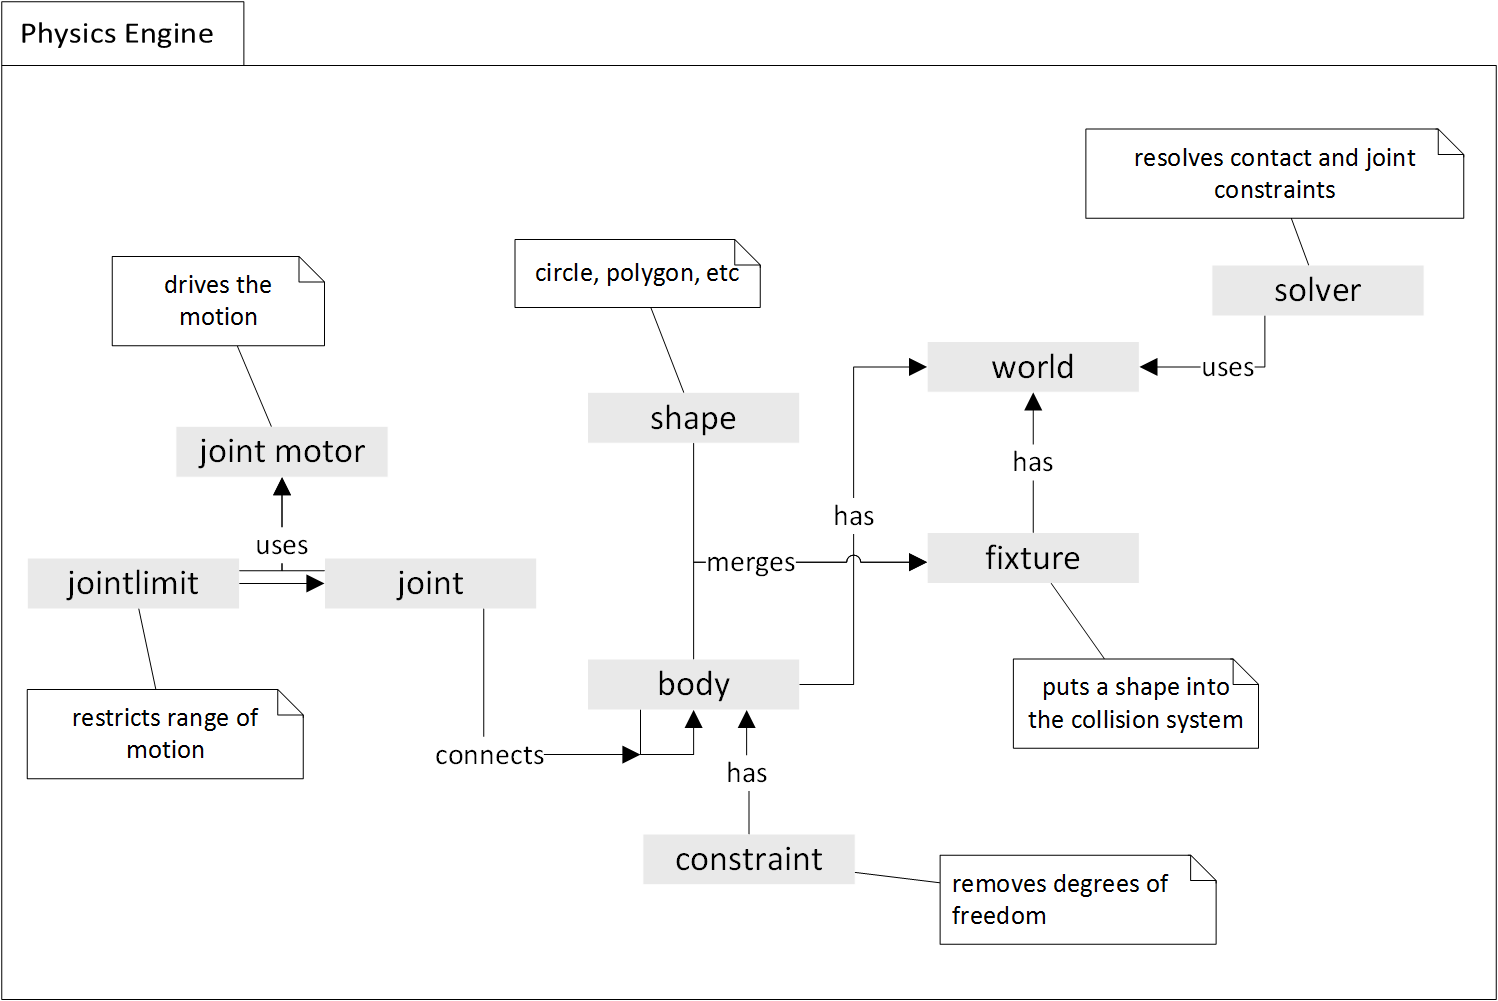
\includegraphics[width=165mm]{Images/physics_overview}
		\caption{Physics Architecture Abstract}
		\label{fig:physics abstract}
	\end{figure}
	
\section{GUI}

	\begin{figure}[h!]
		\centering
		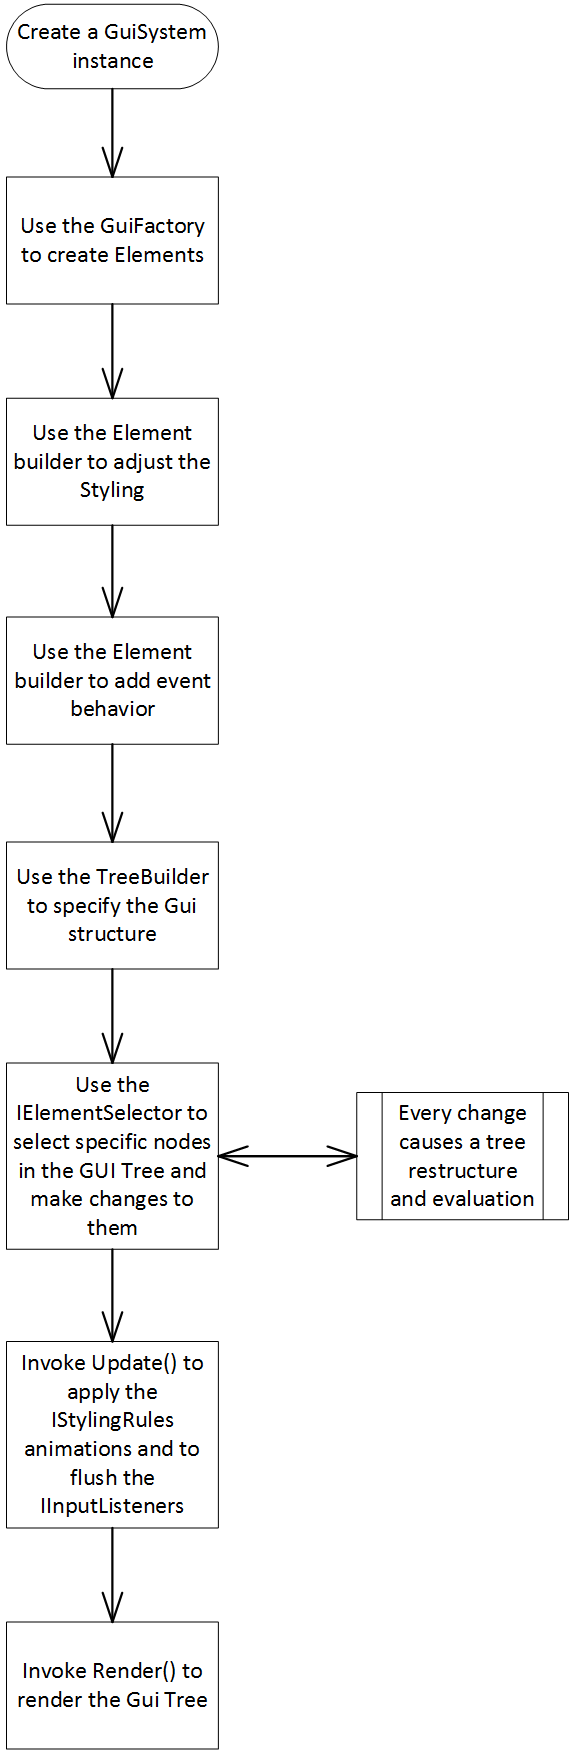
\includegraphics[width=80mm]{Images/gui_usage}
		\caption{Gui Usage Diagram}
		\label{fig:gui_usage}
	\end{figure}
	
	\begin{figure}[h!]
		\centering
		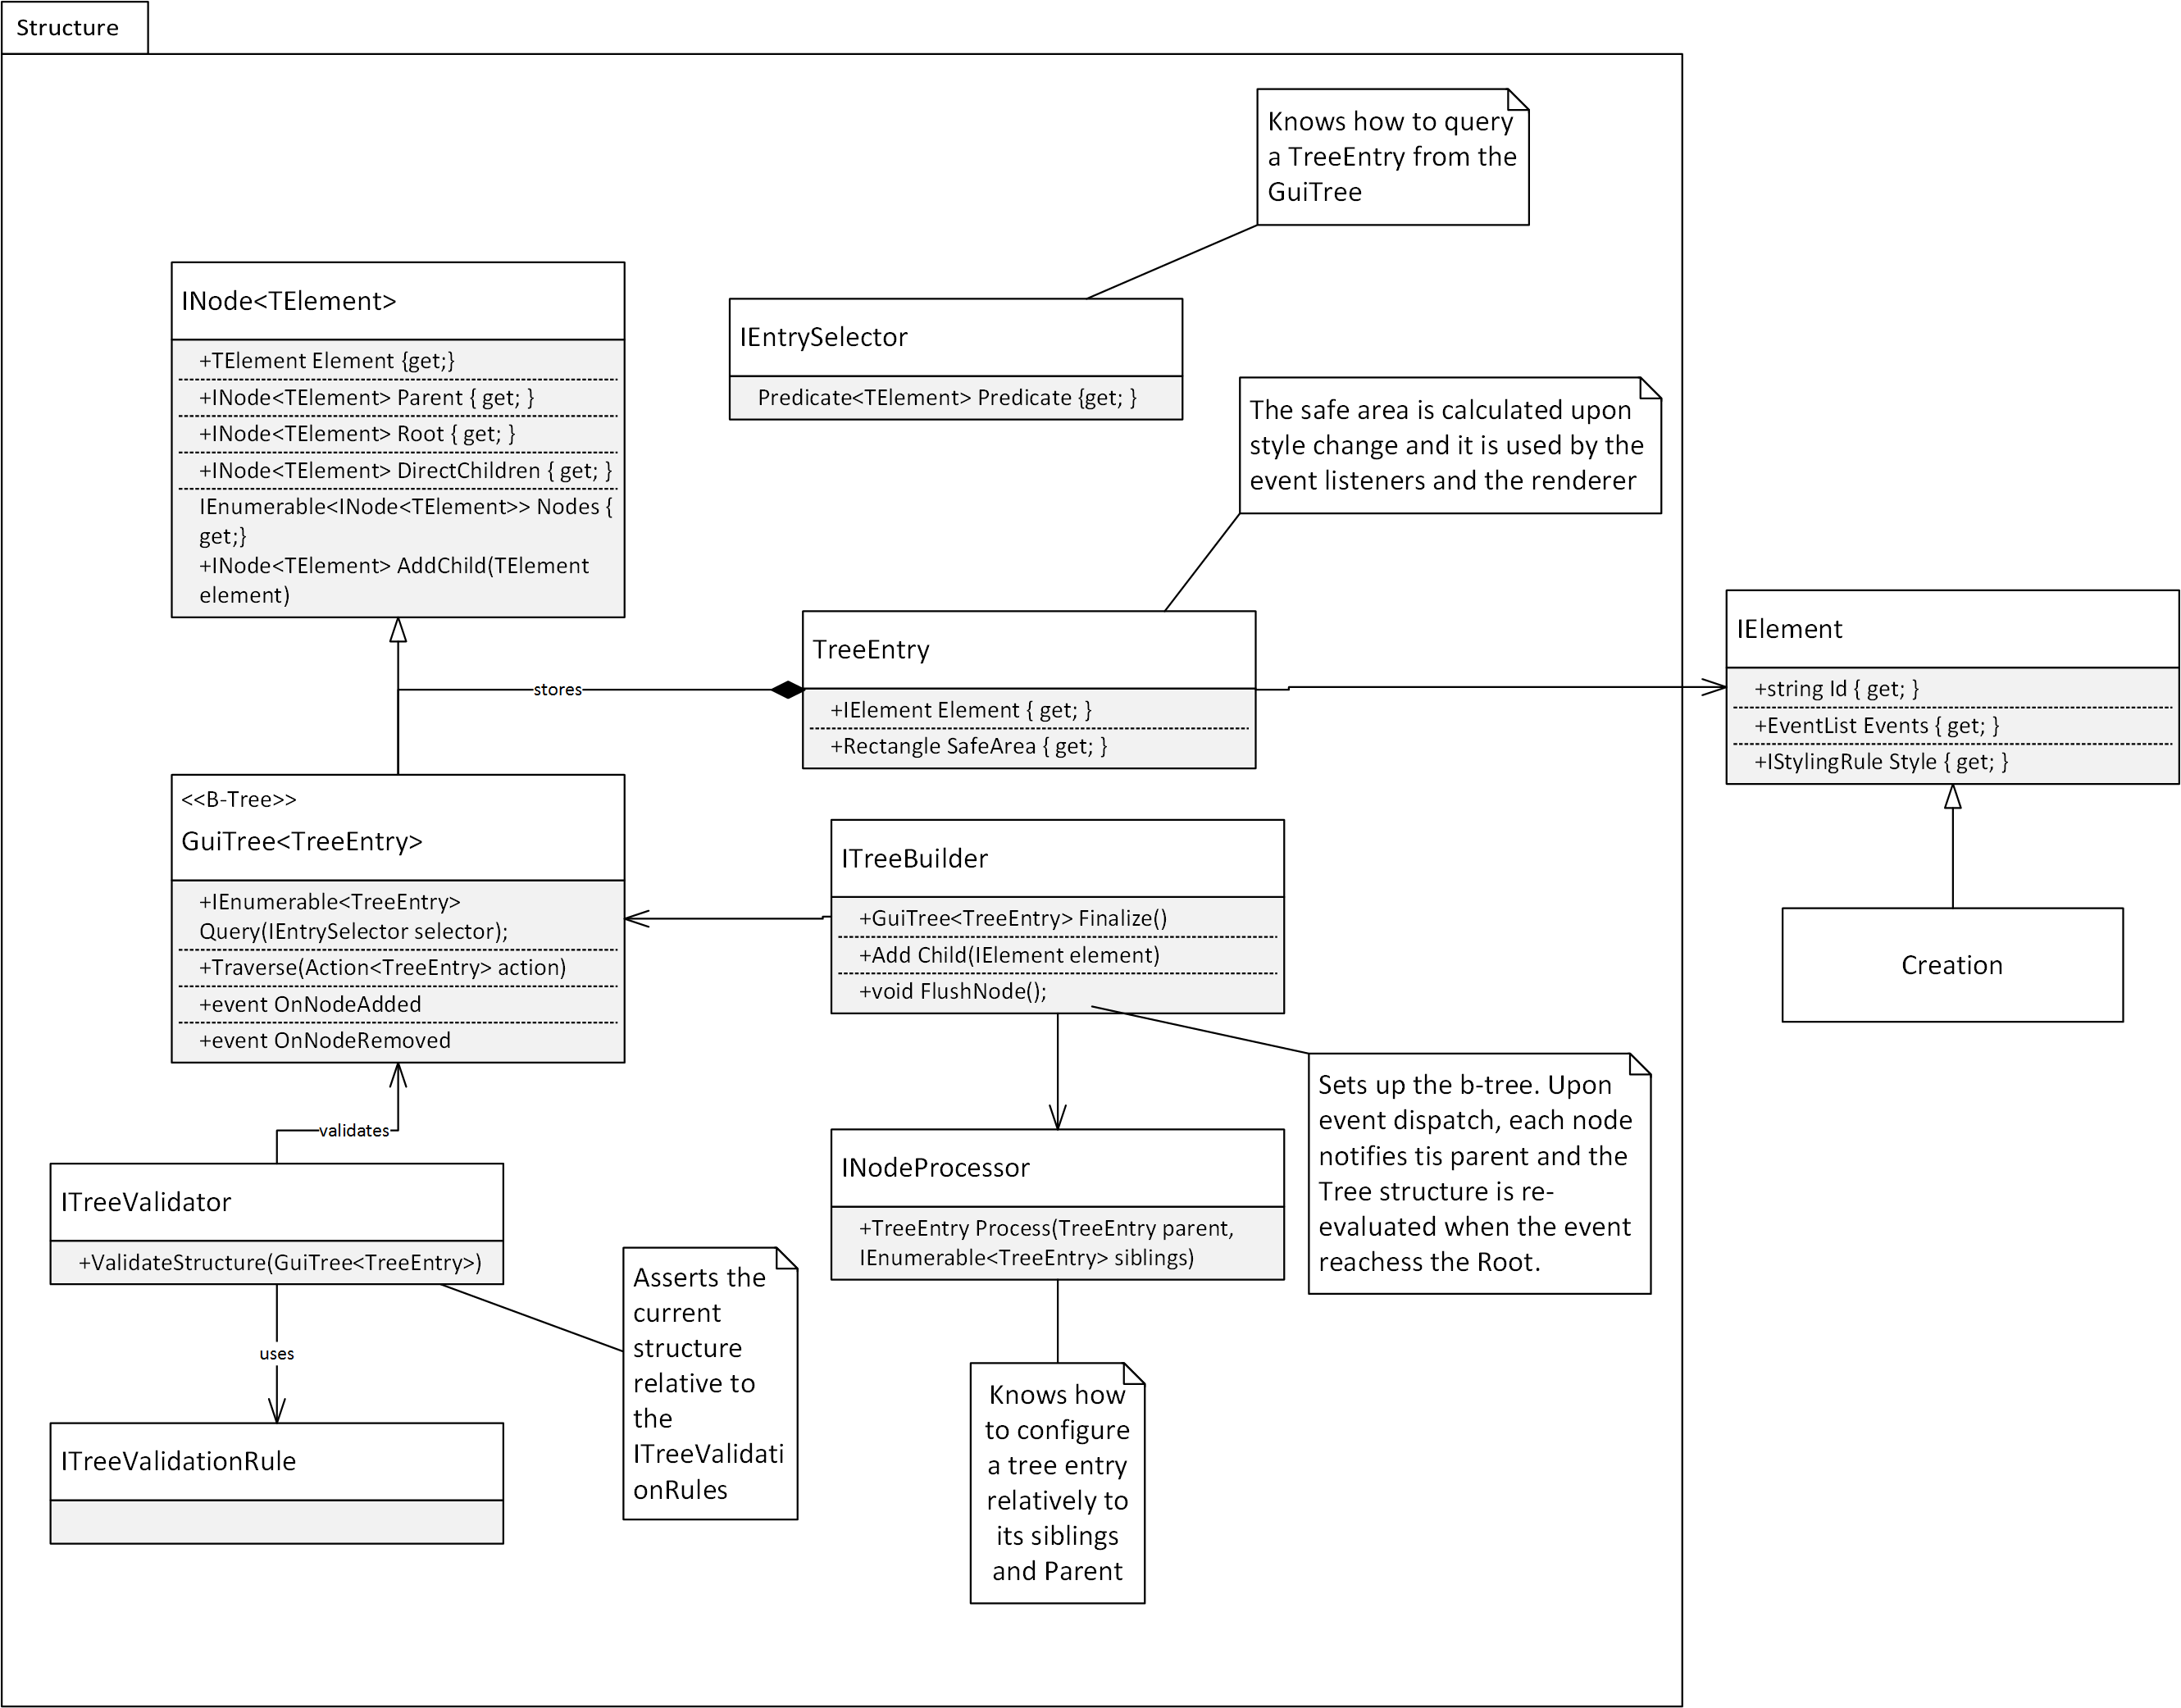
\includegraphics[width=165mm]{Images/gui_structure}
		\caption{Gui Structure Diagram}
		\label{fig:gui_structure}
	\end{figure}
	
	\begin{figure}[h!]
		\centering
		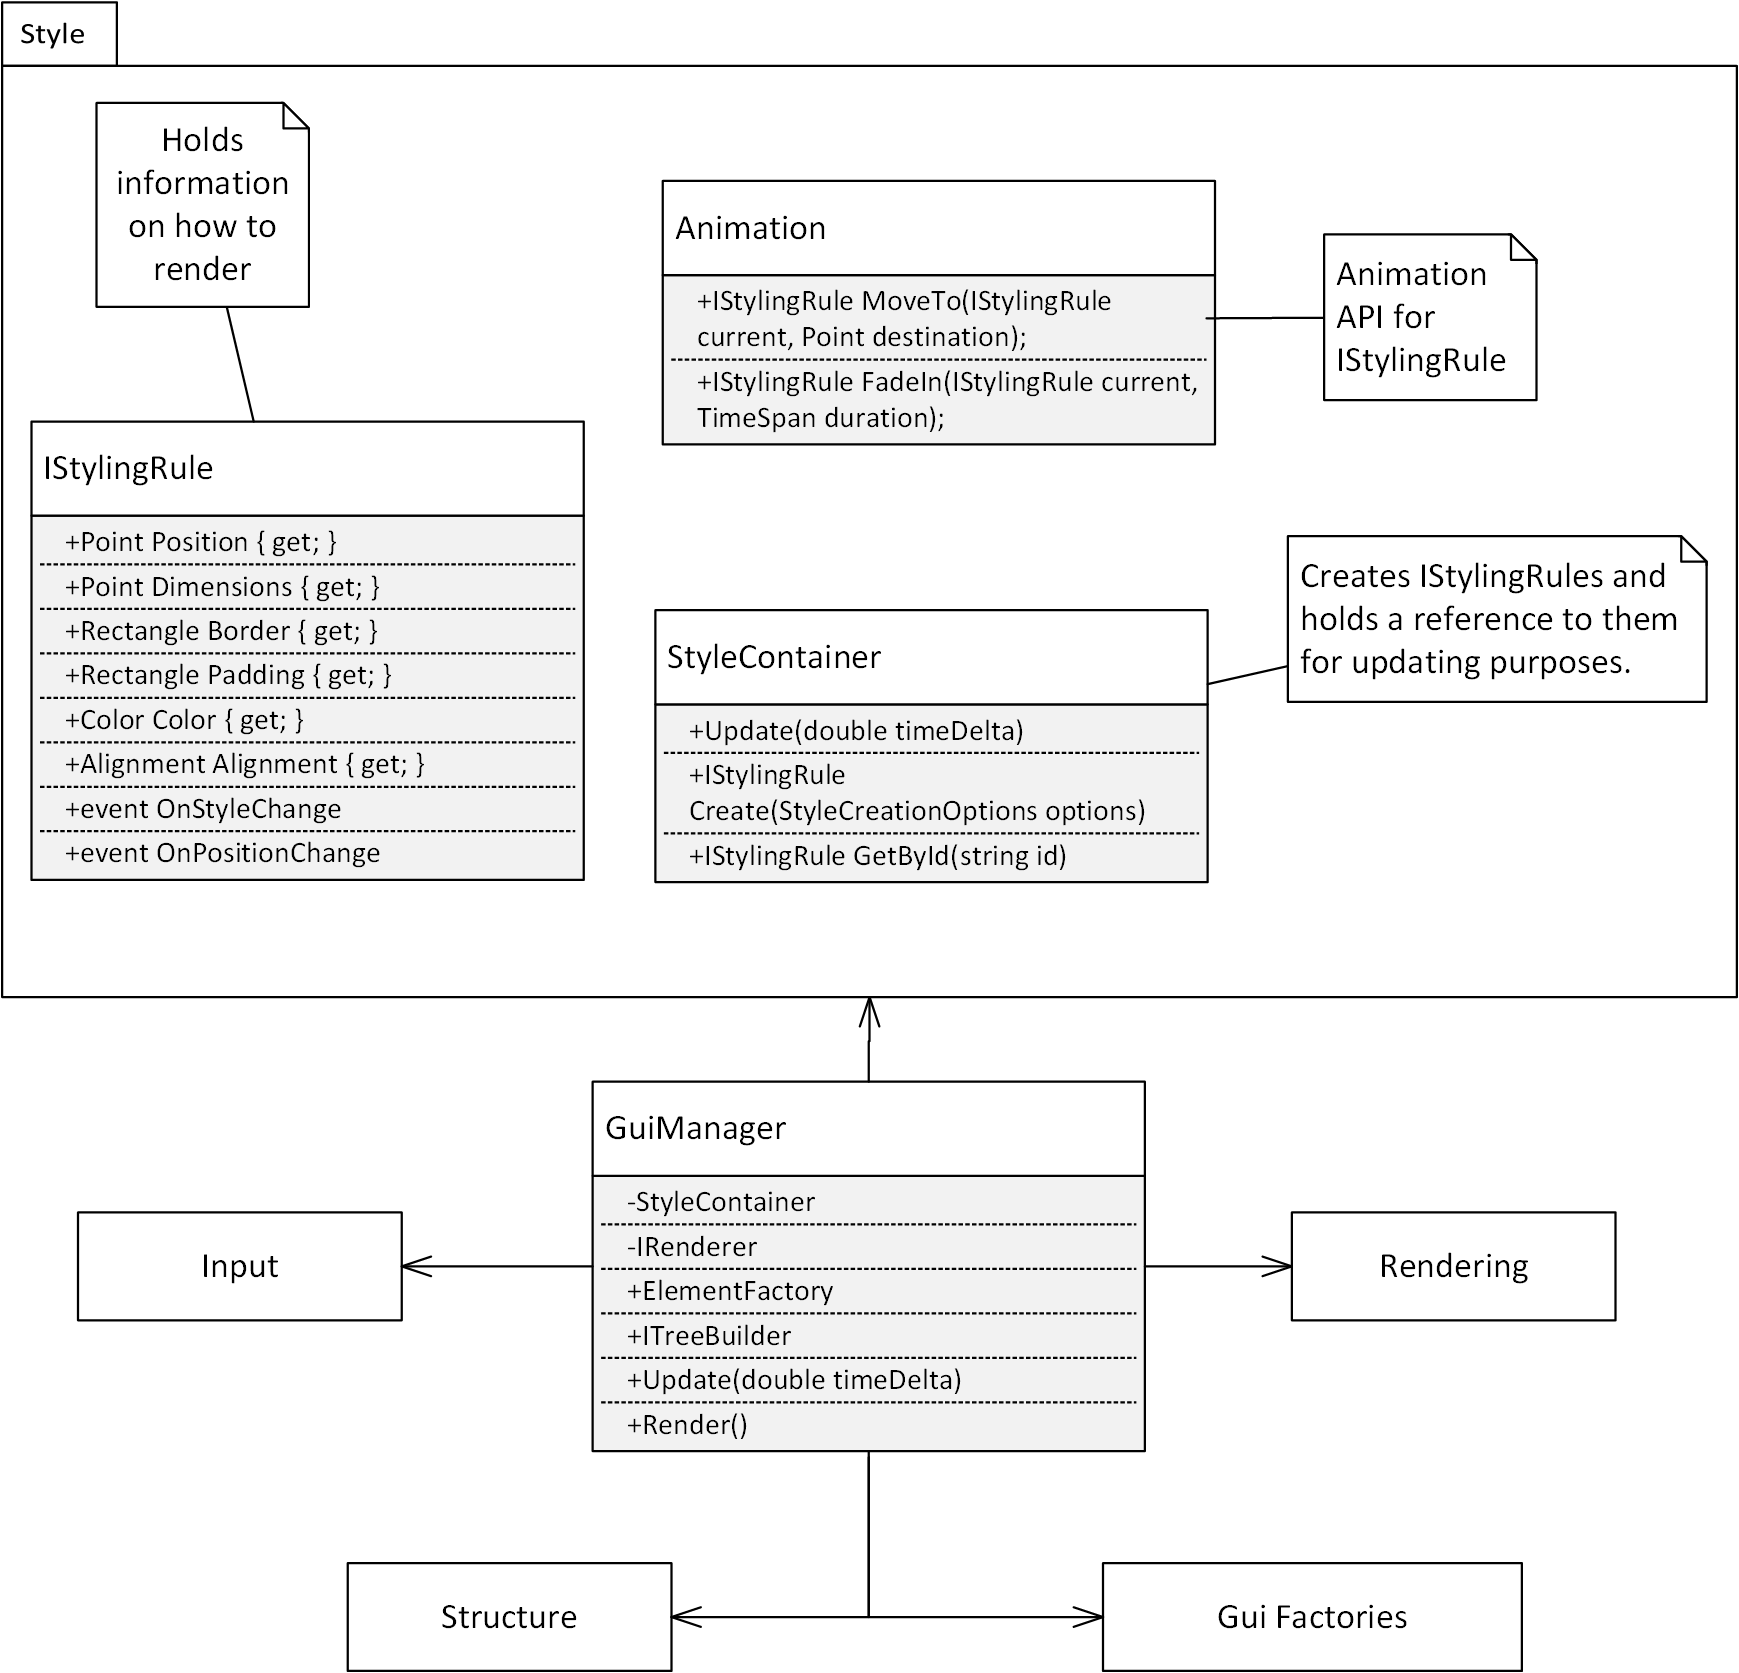
\includegraphics[width=165mm]{Images/gui_system}
		\caption{Gui System Diagram}
		\label{fig:gui_system}
	\end{figure}			